% Drude model implementation of 1D and 2D DNG.
\chapter{FDTD Implementation of Metamaterials Using Dispersive Models}
\section{Limitations of Standard FDTD Algorithm}
Standard FDTD algorithm cannot cater for negative values of permittivity or permeability. This is because of the Courant stability criterion. As soon as the permeability or permittivity becomes less than unity the algorithm will not remain stable. A metamaterial object can be modelled as a dispersive substance using either the Lorentz or Drude dispersive models. These models can yield negative values of permittivity (or permeability) for certain frequency ranges~\cite{NumericalFDTD-Sibel}. Using these dispersive models, FDTD update equations are modified and permittivity and permeabilities are replaced with terms dependent on frequency of operation ($\omega$).
\section{Drude Dispersive Model}
In ideal conditions the permittivity (and permeability) of a material remain constant for any frequency and throughout the structure of that material. Speed of electromagnetic waves in such a medium remain constant if frequency changes. Additionally, there is no loss in energy as the waves pass through the medium. 

In reality, such a material does not exist. Speed of EM waves varies with frequency of operation. Also, there is a loss associated with the material. A material is dispersive if its permittivity or permeability is dependent on frequency~\cite[Ch. 10]{JBSchneiderUFDTD}.

This section follows the treatment of~\cite[Ch. 10, 289--290]{JBSchneiderUFDTD} for deriving permittivity relationship given by Drude model. The Drude model is described by the following second order differential equation that relates the net force on charges moving under the influence of an electric field and facing an impeding force due to collisions with material.
\begin{equation}
\centering
M\dfrac{d^2 \textbf{x}}{dt^2} = Q \textbf{E}(t) - Mg\dfrac{d \textbf{x}}{dt}
\label{Drude-Model-Second-Order-DE}
\end{equation}
The left side of this equation gives mass times acceleration or the net force on charge. Here $M$ is the mass of charge, $Q$ the amount of charge, $\textbf{E}(t)$ is electric field that may vary with time and $g$ is the damping coefficient. Equation~\ref{Drude-Model-Second-Order-DE} can be converted to frequency domain using the relationships $\partial ^2/\partial t^2 \rightarrow (j\omega)^2$ and $\partial/\partial t \rightarrow j\omega$, obtaining,
\begin{equation}
\centering
M(j\omega)^2\hat{\textbf{x}}(\omega)+Mg(j\omega)\hat{\textbf{x}}(\omega)=Q\hat{\textbf{E}}(\omega)
\label{Drude-Model-Second-Order-DE-Frequency-Domain}
\end{equation}
The polarization vector $\textbf{P}$ is given by,
\begin{equation}
\centering
\hat{\textbf{P}}=NQ\hat{\textbf{x}}
\label{Polarization}
\end{equation}
Where, $N$ is the number of dipoles per unit volume. By eliminating $\hat{\textbf{x}}$ from equations~\ref{Drude-Model-Second-Order-DE-Frequency-Domain} and~\ref{Polarization} and rearranging terms polarization can be expressed as,
\begin{equation}
\centering
\hat{\textbf{P}}(\omega)=-\epsilon_0\dfrac{\frac{NQ^2}{M\epsilon_0}}{\omega^2-jg\omega}\hat{\textbf{E}}(\omega)
\label{Polarization-Frequency-Domain}
\end{equation}
By letting $\omega^2_p=NQ^2/M\epsilon_0$, the electric susceptibility is obtained for Drude model as,
\begin{equation}
\centering
\hat{\chi_e}(\omega)=-\dfrac{\omega^2_p}{\omega^2-jg\omega}
\label{Electric-Susceptibility-Drude}
\end{equation}
The relative permittivity in Drude model is expressed as,
\begin{equation}
\centering
\hat{\epsilon_r}(\omega)=\epsilon_\infty-\dfrac{\omega^2_p}{\omega^2-jg\omega}
\label{er-Drude}
\end{equation}
Setting $g=0$ and $\epsilon_\infty=1$, relative permittivity comes out to be negative for $\omega/\omega_p > 1$ (figure~\ref{DrudeModel_er}). Thus, Drude model can be effectively used to model metamaterials with permittivity or permeability less than one by incorporating it into FDTD update equations.
\begin{figure}[H]
\centering
\includegraphics[scale=0.8, trim=4cm 8.5cm 4cm 8.5cm, clip]{FigCh03_DrudeModel_er.pdf}
\caption{$\epsilon_r$ plotted against $\omega/\omega_p$ for $\epsilon_\infty=1$ and $g=0$}
\label{DrudeModel_er}
\end{figure}
\section{FDTD Equations in 1D}
Here, the approach outlined in~\cite{Radial-Zhao} for derivation of FDTD auxiliary update equations is followed. Magnetic field $\textbf{H}$ and magnetic flux density $\textbf{B}$ are related  by the constitutive parameter $\mu$,
\begin{equation}
\centering
\textbf{B} = \mu \textbf{H}
\label{B-mu-H}
\end{equation}
Where, $\mu = \mu_0 \mu_r$. For a lossless, homogeneous, anisotropic and dispersion-less material, relative permeability or $\mu_r$ is a scalar constant. For dispersive material $\mu_r$ is a function of frequency. Similar to equation~\ref{er-Drude}, relative permeability for Drude model is given by,
\begin{eqnarray}
%\centering
\nonumber \hat{\mu_r}(\omega)&=&\mu_\infty-\dfrac{\omega^2_p}{\omega^2-jg\omega}\\
&=&\dfrac{\mu_\infty(\omega^2-jg\omega)-\omega^2_p}{\omega^2-jg\omega}
\label{ur-Drude}
\end{eqnarray}
From equation~\ref{B-mu-H} and~\ref{ur-Drude},
\begin{equation}
\centering
\nonumber \textbf{B} \left( \dfrac{\omega^2-jg\omega}{\mu_\infty(\omega^2-jg\omega)-\omega^2_p} \right) =\textbf{H}
\label{B-muomega-H}
\end{equation}
\begin{equation}
\centering
\omega^2\textbf{B}-g(j\omega)\textbf{B} = \mu_\infty\omega^2\textbf{H}-\omega^2_p\textbf{H}-\mu_\infty g(j\omega)\textbf{H}
\label{B-muomega-H-frequency-domain}
\end{equation}
Frequency domain quantities can be converted to time-domain using the relationships $j\omega \rightarrow \partial/\partial t$ and $\omega^2 \rightarrow - \partial^2/\partial t^2$. Moreover, fields multiplying with $\omega^2_p$ are averaged in time. Second-order difference scheme is used, both for single and double derivatives to keep all the terms in accordance with the second-order nature of whole expression. That would result in easier implementation. Assuming anisotropic nature of material, only $H_y$ and $B_y$ can be considered. Also, $\omega_{pm}$ and $\omega_{pe}$ are used for magnetic and electric field expressions instead of $\omega_p$, whereas, $g_m$ and $g_e$ are used for magnetic and electric collision frequencies, respectively.
\begin{eqnarray}
\nonumber \left(\dfrac{B^{n+1}_y-2B^n_y+B^{n-1}_y}{(\Delta t)^2}\right) &+& g_m\left(\dfrac{B^{n+1}_y-B^{n-1}_y}{2\Delta t}\right) =\\
\nonumber &&\mu_0\mu_\infty\left(\dfrac{H^{n+1}_y-2H^n_y+H^{n-1}_y}{(\Delta t)^2}\right)+\\
\nonumber && \mu_0\omega^2_{pm}\left(\dfrac{H^{n+1}_y+2H^n_y+H^{n-1}_y}{4}\right)+\\
&& \mu_0\mu_\infty g_m\left(\dfrac{H^{n+1}_y-H^{n-1}_y}{2\Delta t}\right)
\label{2nd-order-B-H}
\end{eqnarray}
By separating $H^{n+1}_y$ the final form of equation is,
\begin{eqnarray}
\nonumber H^{n+1}_y &=& a_m\left(B^{n+1}_y-2B^n_y+B^{n-1}_y\right)+b_m\left(B^{n+1}_y-B^{n-1}_y\right)+\\
&&c_m\left(2H^n_y-H^{n-1}_y\right)+d_m\left(2H^n_y+H^{n-1}_y\right)+e_m H^{n-1}_y
\label{2nd-order-B-H-final-form}
\end{eqnarray}
Where,
\begin{eqnarray}
\nonumber & a_m=\dfrac{4}{4\mu_0\mu_\infty+\mu_0\omega^2_{pm}\left(\Delta t\right)^2+\mu_0\mu_\infty g_m \left(2\Delta t\right)}\\
\nonumber & b_m=\dfrac{g_m\left(2\Delta t\right)}{4\mu_0\mu_\infty+\mu_0\omega^2_{pm}\left(\Delta t\right)^2+\mu_0\mu_\infty g_m \left(2\Delta t\right)}\\
\nonumber & c_m=\dfrac{4\mu_0\mu_\infty}{4\mu_0\mu_\infty+\mu_0\omega^2_{pm}\left(\Delta t\right)^2+\mu_0\mu_\infty g_m \left(2\Delta t\right)}\\
\nonumber & d_m=\dfrac{-\mu_0\omega^2_{pm}\left(\Delta t\right)^2}{4\mu_0\mu_\infty+\mu_0\omega^2_{pm}\left(\Delta t\right)^2+\mu_0\mu_\infty g_m \left(2\Delta t\right)}\\
\nonumber & e_m=\dfrac{\mu_0\mu_\infty g_m\left(2\Delta t\right)}{4\mu_0\mu_\infty+\mu_0\omega^2_{pm}\left(\Delta t\right)^2+\mu_0\mu_\infty g_m \left(2\Delta t\right)}
\label{1D-Drude-H-scalars}
\end{eqnarray}
A similar derivation can be carried out to derive the auxiliary update equation for electric field given by,
\begin{eqnarray}
\nonumber E^{n+1}_x &=& a_e\left(D^{n+1}_x-2D^n_x+D^{n-1}_x\right)+b_e\left(D^{n+1}_x-D^{n-1}_x\right)+\\
&&c_e\left(2E^n_x-E^{n-1}_x\right)+d_e\left(2E^n_x+E^{n-1}_x\right)+e_e E^{n-1}_x
\label{2nd-order-D-E-final-form}
\end{eqnarray}
Where,
\begin{eqnarray}
\nonumber & a_e=\dfrac{4}{4\epsilon_0\epsilon_\infty+\epsilon_0\omega^2_{pe}\left(\Delta t\right)^2+\epsilon_0\epsilon_\infty g_e \left(2\Delta t\right)}\\
\nonumber & b_e=\dfrac{g_e\left(2\Delta t\right)}{4\epsilon_0\epsilon_\infty+\epsilon_0\omega^2_{pe}\left(\Delta t\right)^2+\epsilon_0\epsilon_\infty g_e \left(2\Delta t\right)}\\
\nonumber & c_e=\dfrac{4\epsilon_0\epsilon_\infty}{4\epsilon_0\epsilon_\infty+\epsilon_0\omega^2_{pe}\left(\Delta t\right)^2+\epsilon_0\epsilon_\infty g_e \left(2\Delta t\right)}\\
\nonumber & d_e=\dfrac{-\epsilon_0\omega^2_{pe}\left(\Delta t\right)^2}{4\epsilon_0\epsilon_\infty+\epsilon_0\omega^2_{pe}\left(\Delta t\right)^2+\epsilon_0\epsilon_\infty g_e \left(2\Delta t\right)}\\
\nonumber & e_e=\dfrac{\epsilon_0\epsilon_\infty g_e\left(2\Delta t\right)}{4\epsilon_0\epsilon_\infty+\epsilon_0\omega^2_{pe}\left(\Delta t\right)^2+\epsilon_0\epsilon_\infty g_e \left(2\Delta t\right)}
\label{1D-Drude-E-scalars}
\end{eqnarray}
For a wave propagating in $z$ direction, FDTD update equations are,
\begin{equation}
B^{n+1}_y(k)=B^n_y(k)+\dfrac{\Delta t}{\Delta z}\left(E^n_x(k)-E^n_x(k+1)\right)
\label{1D-B-Update-Equation}
\end{equation}
\begin{equation}
D^{n+1}_x(k)=D^n_x(k)+\dfrac{\Delta t}{\Delta z}\left(H^{n+1}_y(k-1)-H^{n+1}_y(k)\right)
\label{1D-D-Update-Equation}
\end{equation}
Equations \ref{1D-B-Update-Equation} and \ref{1D-D-Update-Equation} drive the FDTD algorithm which give future values of $By$ and $Dx$ from past fields. Equations \ref{2nd-order-B-H-final-form} and \ref{2nd-order-D-E-final-form} are auxiliary equations which give future fields $H_y$ and $E_x$ at $n+1$.
\section{Simulation of 1D DNG Slab}
\subsection{Problem Specification}
An electromagnetic wave travelling in $z$ direction is incident on a slab with negative values of permittivity and permeability (DNG) at the frequency of operation \cite{DNG-Ehud-Ziol}. Sinusoidal wave, Gaussian pulse and Ricker wavelet are used as sources. Transmission and reflection coefficients are calculated at the air-slab interface. Refractive index of slab for a range of frequencies is also computed. By varying parameters, the simulation can be scaled to any desired frequency or wavelength. Matlab code of this simulation is given in appendix C.
\subsection{Implementation Details}
There are three main phases in the implementation:
\begin{enumerate}
\item Initialisation
\item Simulation
\item Post-processing
\end{enumerate}
Figure \ref{1D-DNG-Algorithm} depicts the flow of program.
\subsection{Initialisation}
In this phase, simulation parameters are specified. Simulation parameters are total number of spatial steps, time steps, wavelength and frequency of operation etc. Field arrays are then allocated and initialised. Any additional fields that are required for post-processing are also initialised. Arrays containing $g_m$, $g_e$, $\omega^2_{pm}$ and $\omega^2_{pe}$ must be initialised with values specified for each location in the domain.
\subsection{Simulation}
A dry run must carried out without any obstacle if reflection coefficient is to be calculated in order to record the incident field where obstacle is to be placed. The actual simulation consists of five steps:
\begin{enumerate}
\item Compute future value of $B_y$ from past values of $B_y$ and $E_x$ (equation \ref{1D-B-Update-Equation}).
\item Compute future value of $H_y$ from $B_y$ calculated in step 1 (equation \ref{2nd-order-B-H-final-form}).
\item Compute future value of $D_x$ from past value of $D_x$ and $H_y$ in step 2 (equation \ref{1D-D-Update-Equation}).
\item Compute future value of $E_x$ from $D_x$ calculated in step 3 (equation \ref{2nd-order-D-E-final-form}).
\item Update additive source at specified source location for current time step.
\end{enumerate}
Electric field snapshots are saved at specified intervals during simulation and played-back as a movie after simulation ends. 
\subsection{Post-processing}
After the simulation ends, reflection and transmission coefficients are calculated at the air-slab interface. Refractive index is calculated in the slab. A time-domain movie of the simulation is played that shows incident wave passing through the slab and undergoing dispersion.
\begin{figure}[htbp]
\centering
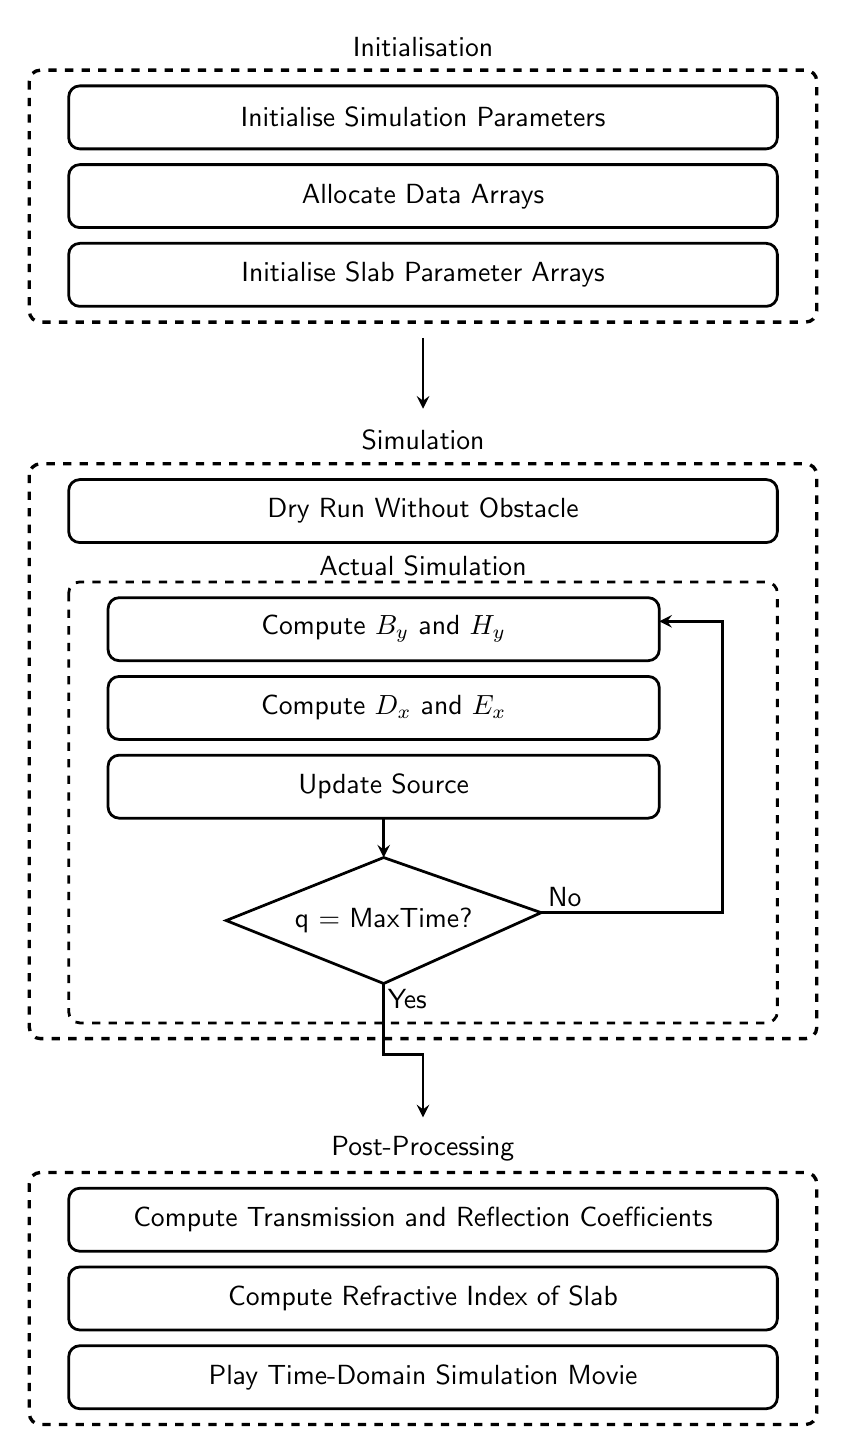
\begin{tikzpicture}
	% Initialisation.
	\draw (5cm,0.1cm) node {\textsf{Initialisation}};
	% Large dashed rectangle.
	\draw[line width=1.2pt, rounded corners, dashed] (0cm,-0.2cm) rectangle (10cm,-3.4cm);
	% Simulation parameters.
	\draw[line width=1pt, rounded corners] (0.5cm,-0.4cm) rectangle (9.5cm,-1.2cm);
	\draw (5cm,-0.8cm) node {\textsf{Initialise Simulation Parameters}};
	% Allocate data arrays.
	\draw[line width=1pt, rounded corners] (0.5cm,-1.4cm) rectangle (9.5cm,-2.2cm);
	\draw (5cm,-1.8cm) node {\textsf{Allocate Data Arrays}};
	% Initialise slab parameter arrays.
	\draw[line width=1pt, rounded corners] (0.5cm,-2.4cm) rectangle (9.5cm,-3.2cm);
	\draw (5cm,-2.8cm) node {\textsf{Initialise Slab Parameter Arrays}};
	\draw[line width=1pt, ->, >=stealth] (5cm,-3.6cm) -- (5cm,-4.5cm);

	% Simulation.
	\draw (5cm,-4.9cm) node {\textsf{Simulation}};
	% Large dashed rectangle.
	\draw[line width=1.2pt, rounded corners, dashed] (0cm,-5.2cm) rectangle (10cm,-12.5cm);
	% Dry run without obstacle.
	\draw[line width=1pt, rounded corners] (0.5cm,-5.4cm) rectangle (9.5cm,-6.2cm);
	\draw (5cm,-5.8cm) node {\textsf{Dry Run Without Obstacle}};
	% Actual Simulation.
	\draw[line width=1pt, rounded corners, dashed] (0.5cm,-6.7cm) rectangle (9.5cm,-12.3cm);
	\draw (5cm,-6.5cm) node {\textsf{Actual Simulation}};
	% Compute H fields.
	\draw[line width=1pt, rounded corners] (1.0cm,-6.9cm) rectangle (8.0cm,-7.7cm);
	\draw (4.5cm,-7.3cm) node {\textsf{Compute $B_y$ and $H_y$}};
	% Compute E fields.
	\draw[line width=1pt, rounded corners] (1.0cm,-7.9cm) rectangle (8.0cm,-8.7cm);
	\draw (4.5cm,-8.3cm) node {\textsf{Compute $D_x$ and $E_x$}};
	% Apply source.
	\draw[line width=1pt, rounded corners] (1.0cm,-8.9cm) rectangle (8.0cm,-9.7cm);
	\draw (4.5cm,-9.3cm) node {\textsf{Update Source}};
	\draw[line width=1pt, ->, >=stealth] (4.5cm,-9.7cm) -- (4.5cm,-10.2cm);
	% Diamond.
	\draw[line width=1pt] (4.5cm,-10.2cm) -- (2.5cm,-11cm) -- (4.5cm,-11.8cm) -- (6.5cm,-10.9cm) -- cycle;
	\draw (4.5cm,-11cm) node {\textsf{q = MaxTime?}};
	% No?
	\draw[line width=1pt, ->, >=stealth] (6.5cm,-10.9cm) -- (8.8cm,-10.9cm) -- (8.8cm,-7.2cm) -- (8.0cm,-7.2cm);
	\draw (6.8cm,-10.7cm) node {\textsf{No}};
	% Yes?
	\draw[line width=1pt, ->, >=stealth] (4.5cm,-11.8cm) -- (4.5cm,-12.7cm) -- (5cm,-12.7cm) -- (5cm,-13.5cm);
	\draw (4.8cm,-12.0cm) node {\textsf{Yes}};

	% Post-processing.
	\draw (5cm,-13.9cm) node {\textsf{Post-Processing}};
	% Large dashed rectangle.
	\draw[line width=1.2pt, rounded corners, dashed] (0cm,-14.2cm) rectangle (10cm,-17.4cm);
	% Transmission/Reflection coefficient calculations.
	\draw[line width=1pt, rounded corners] (0.5cm,-14.4cm) rectangle (9.5cm,-15.2cm);
	\draw (5cm,-14.8cm) node {\textsf{Compute Transmission and Reflection Coefficients}};
	% Refractive index calculations.
	\draw[line width=1pt, rounded corners] (0.5cm,-15.4cm) rectangle (9.5cm,-16.2cm);
	\draw (5cm,-15.8cm) node {\textsf{Compute Refractive Index of Slab}};
	% Simulation movie.
	\draw[line width=1pt, rounded corners] (0.5cm,-16.4cm) rectangle (9.5cm,-17.2cm);
	\draw (5cm,-16.8cm) node {\textsf{Play Time-Domain Simulation Movie}};
\end{tikzpicture}
\caption{Simulation algorithm}
\label{1D-DNG-Algorithm}
\end{figure}
\section{Simulation Results}
The simulation was run for both lossless and lossy cases with sinusoidal, Gaussian and Ricker wavelet sources. The slab parameters was set such that at frequency of operation, $f_0$, the permittivity and permeability of slab are both negative and resulted in a refractive index $n=-1$.
\subsection{Simulation Parameters}
The number of spatial steps was set as $4096$ and simulation was run for $4096$ time steps. The slab was located between steps $1365$ and $2731$. $\Delta z$ or spatial step was set as $3$ mm and time step, $\Delta t$, was set as $50$ ps. Frequency of operation was $f_0=0.1953125$ GHz and Courant number for this configuration was $S_c=0.5$. In order to obtain relative permittivity and permeability of $-1$ at required $f_0$, plasma frequencies were set as $\omega^2_{pm}=\omega^2_{pe}=2\times(2\pi f_0)^2$ with $\epsilon_\infty=\mu_\infty=1$.
\subsection{Incident and Transmitted Fields}
Simulation with Gaussian pulse revealed that low frequency components were reflected at the interface which was confirmed from the transmission and reflection coefficients obtained for the air-slab interface. At $f_0$, the transmission coefficient was $1$ and there were no reflections when a sinusoidal source with $f_0$ was incident on the slab. Under steady-state conditions, transmitted wave inside the slab had negative phase velocity while energy was propagating in $+\hat{z}$ direction as expected.
\subsection{Refractive Index}
Following \cite{DNG-Ehud-Ziol}, the refractive index was calculated from,
\begin{equation}
n_{FDTD} = \dfrac{1}{jk_0(z_1-z_2)}log\left|\dfrac{E_x(\omega,z_2)}{E_x(\omega,z_1)}\right|
\label{Refractive-Index-FDTD}
\end{equation}
Where, $k_0$ was the wave number set as $\omega_0/c$ and the fields were recorded at locations $z_1=1415\Delta z$ and $z_2=1424\Delta z$. For both, Gaussian pulse and Ricker wavelet, $Re(n)$ was $-1$ at $f_0$ while $Im(n)$ was sufficiently close to $0$.
\begin{figure}[H]
\centering
\includegraphics[scale=0.8, trim=3.5cm 8.7cm 4.5cm 8.85cm, clip]{FigCh03_IncidentFieldGaussian.pdf}
\caption{Gaussian pulse}
\label{1DDNG-IncidentField-Gaussian}
\end{figure}
\begin{figure}[H]
\centering
\includegraphics[scale=0.8, trim=3.5cm 8.7cm 4.5cm 8.85cm, clip]{FigCh03_IncidentFieldRicker.pdf}
\caption{Ricker wavelet}
\label{1DDNG-IncidentField-Ricker}
\end{figure}
\begin{figure}[H]
\centering
\includegraphics[scale=0.8, trim=3.5cm 8.7cm 4.5cm 8.85cm, clip]{FigCh03_IncidentFieldSinusoidal.pdf}
\caption{Sinusoidal wave}
\label{1DDNG-IncidentField-Sinusoidal}
\end{figure}
\begin{figure}[H]
\centering
\includegraphics[scale=0.8, trim=3.5cm 8.7cm 4.5cm 8.85cm, clip]{FigCh03_TransmissionReflectionCoefficient.pdf}
\caption{Transmission and reflection coefficients}
\label{1DDNG-Transmission-Reflection-Coefficient}
\end{figure}
\begin{figure}[H]
\centering
\includegraphics[scale=0.8, trim=3.5cm 8.7cm 4.5cm 8.85cm, clip]{FigCh03_TransmittedField.pdf}
\caption{Transmitted Gaussian pulse}
\label{1DDNG-Transmitted-Gaussian-Pulse}
\end{figure}
\begin{figure}[H]
\centering
\subfigure{\includegraphics[scale=0.8, trim=3.5cm 8.7cm 4.5cm 8.85cm, clip]{FigCh03_RefractiveIndex.pdf}}
\subfigure{\includegraphics[scale=0.8, trim=3.5cm 8.7cm 4.5cm 8.85cm, clip]{FigCh03_RefractiveIndexZoomed.pdf}}
\caption{Refractive index}
\label{1DDNG-Refractive-Index}
\end{figure}
\begin{figure}[H]
\centering
\includegraphics[scale=0.78, trim=3.5cm 8.7cm 4.5cm 8.75cm, clip]{FigCh03_1DDNGSteadyStateLossless.pdf}
\caption{Steady-state under lossless conditions}
\label{1DDNG-SteadyState-Lossless}
\end{figure}
\begin{figure}[H]
\centering
\includegraphics[scale=0.78, trim=3.5cm 8.7cm 4.5cm 8.75cm, clip]{FigCh03_1DDNGSteadyStateLossy.pdf}
\caption{Steady-state under lossy conditions}
\label{1DDNG-SteadyState-Lossy}
\end{figure}